Since $f$ and $g$ have the same principal parts, their difference $f - g$ is holomorphic on $\C$. Therefore, if we can show that $f - g$ is bounded we will be able to use Liouville's theorem to conclude that it is constant. We first show that $\abs{f(z)} \to 0$ as $\Im(z) = y \to \infty$ uniformly with respect to $x$. This means that for any $\epsilon > 0$ we can find $b > 0$ such that for $\abs{y} \geq b$ we have $\abs{f(z)} < \epsilon$. By periodicity of $f$, it suffices to show this on a vertical strip of width 1.

Suppose $z$ is in a strip of width 1 where its imaginary part $y$ satisfies $\abs{y} > b$ for some $b > 0$. Notice that the terms of the series are holomorphic on this subset and converge uniformly and absolutely on compact subsets. 
% Moreover each of the terms $1/(z - n)^2$ goes to 0 uniformly with respect to $x$ as $\abs{y} \to \infty$. 
There is some large $N$ such that for all $z$ we have
$$\sum_{\abs{n} > N} \frac{1}{\abs{z - n}^2} < \frac{\epsilon}{2}$$
as this the tail of a convergent series. 

The finitely many terms in the sum that remain also go to 0 uniformly with respect to $x$ and can individually be bounded (in particular we choose $b$ so that all the remaining terms are small). To be precise, for every $|n| \leq N$, we consider $1/(z - n)^2$ which goes to 0 uniformly as $\abs{y} \to \infty$. In particular then there exists some $b_n$ such that if $\abs{y} > b_n$ then $\abs{1/(z - n)^2} < \epsilon/4N$. Now we take $b$ to be greater than all these $b_n$. Then notice that for $\abs{y} > b$ we have 
\begin{align*}
    \sum_{n = -\infty}^{\infty} \frac{1}{\abs{z - n}^2} &= \sum_{n = -N}^N \frac{1}{\abs{z - n}^2} + \sum_{\abs{n} > N} \frac{1}{\abs{z - n}^2}\\
    &< \sum_{n = -N}^N \frac{\epsilon}{4N} + \frac{\epsilon}{2}\\
    &= \epsilon
\end{align*} 
Notice that $g$ also has this property since 
$$\abs{\sin(\pi z)}^2 = \sin^2 (\pi x) + \sinh^2 (\pi y)$$

Now it is easy to see that $f - g$ is bounded. In particular on any strip, $f - g$ is bounded for $\abs{y} \leq b$ by compactness and we know the difference goes to 0 for $\abs{y} > b$. Therefore $f - g$ must be a constant and since the limit is 0 as $\abs{y} \to \infty$, the constant must be 0.

\subsubsection{Example 2}
For a second example consider the series
$$f(z) := \frac{1}{z} + \sum_{n \neq 0} \left( \frac{1}{z - n} + \frac{1}{n} \right)$$
The series does indeed converge on compact subsets of $\C$ (to a meromorphic function which we prematurely called $f$) since each term in the series is of the form $z/n(z - n)$ which is comparable to $1/n^2$ (on compact sets because we can bound $z$). Moreover if we differentiate the series for $f$ term by term we get
\begin{align*}
    f'(z) &= -\frac{1}{z^2} - \sum_{n \neq 0} \frac{1}{(z - n)^2}\\
    &= -\sum_{n = -\infty}^\infty \frac{1}{(z - n)^2}\\
    &= - \left( \frac{\pi}{\sin(\pi z)} \right)^2\\
    &= \frac{d}{dz} \pi \cot(\pi z)
\end{align*}
Therefore $f(z) - \pi \cot(\pi z)$ is a constant (since their derivatives are equal) and this constant must be 0 since the functions are odd. Therefore
\begin{align*}
    \frac{1}{z} + \sum_{n \neq 0} \frac{1}{z - n} + \frac{1}{n} = \pi \cot(\pi z)
\end{align*}

\section{Weierstrass $\wp$-function}
We say a function $f(z)$ is doubly periodic if it is periodic with respect to a discrete subgroup $\Gamma$ of $\C$ with 2 generators. This means that $f(z + \omega) = f(z)$ for every $\omega \in \Gamma$ for a subgroup $\Gamma$ of the form 
$$\Gamma = \{n_1 e_1 + n_2 e_2 : n_1, n_2 \in \Z\}$$
where $e_1, e_2$ are complex numbers are linearly independent over $\R$ (see \autoref{fig:lattice-in-cmplx-plane}). Equivalently, one can say that $f$ has $\Gamma$ as its group of periods.

\begin{figure}[ht]
    \centering
    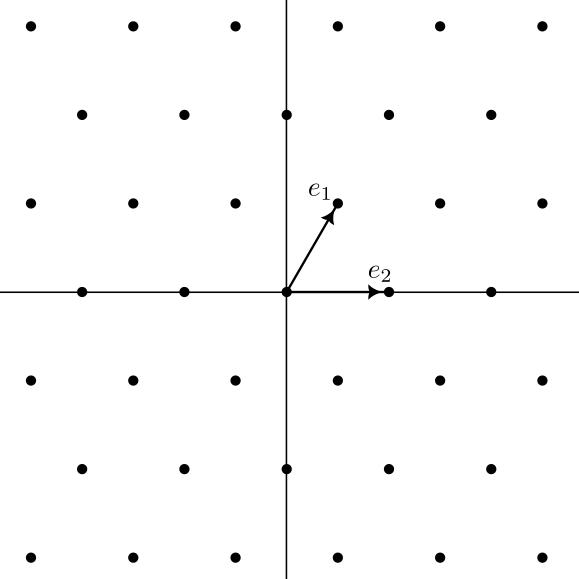
\includegraphics{Images/lattice_in_cmplx_plane.png}
    \caption{$\Gamma$ is a discrete subgroup or lattice of $\C$}
    \label{fig:lattice-in-cmplx-plane}
\end{figure}


The Weierstrass $\wp$ function is defined with respect to a group of periods. So let $\Gamma$ be a discrete subgroup of $\C$ as described above. Then
$$\wp(z) = \frac{1}{z^2} + \sum_{w \in \Gamma \setminus \{0\}} \left( \frac{1}{(z - \omega)^2} - \frac{1}{\omega^2} \right)$$
We claim that this is uniformly and absolutely convergent on compact subsets of $\C$. In order to see this, we first need the following lemma.
\begin{lemma}
Given a discrete subgroup $\Gamma$, we have 
$$\sum_{\omega \in \Gamma \setminus \{0\}} \frac{1}{\abs{\omega}^3} < \infty$$
\end{lemma}
\begin{proof}
    In order to verify that the sum converges, we will sum over the points in a clever way, from the center outwards in a radial manner. Let $P_n = \{t_1 e_1 + t_2 e_2 : \max\{t_1, t_2\} = n\}$. These are the $8n$ points that lie on the $n$-th parallelogram from the middle. Let $k$ be the minimum distance between the origin and $P_1$. Then the distance between the origin and $P_2$ is $2k$ and in general the distance between the origin and $P_n$ is $nk$ (see \autoref{fig:weierstrass-p-grid}). Therefore 
    \begin{align*}
        \sum_{\omega \in \Gamma \setminus \{0\}} \frac{1}{\abs{\omega}^3} &= \sum_{n = 1}^\infty \sum_{\omega \in P_n} \frac{1}{\abs{\omega}^3}\\
        &\leq \sum_{n = 1}^\infty 8n \cdot \frac{1}{(nk)^3}\\
        &= \sum_{n = 1}^\infty \frac{8}{n^2 k^3}
    \end{align*}
    and we know the final series converges.
    \begin{figure}[ht]
        \centering
        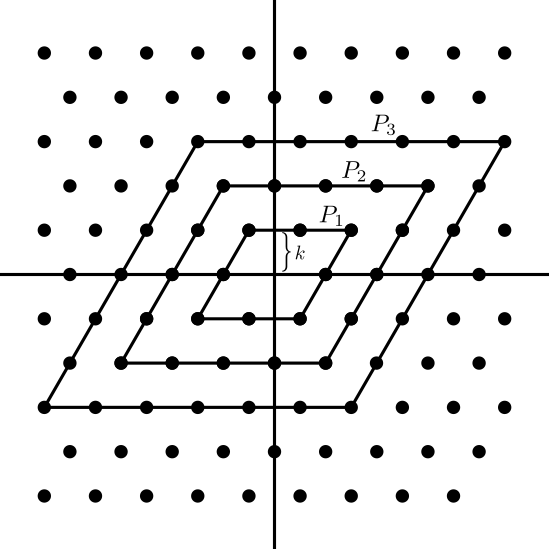
\includegraphics[scale=0.9]{Images/weierstrass_p_grid.png}
        \caption{Sum `radially' from the origin}
        \label{fig:weierstrass-p-grid}
    \end{figure}
\end{proof}

\begin{proposition}
Given a discrete subgroup $\Gamma \subset \C$, the series
$$\frac{1}{z^2} + \sum_{\omega \in \Gamma \setminus \{0\}} \frac{1}{(z - \omega)^2} - \frac{1}{\omega^2}$$
converges absolutely and uniformly on compact subsets of $\C$.
\end{proposition}
\begin{proof}
    It suffices to show that the series converges on closed disks $\abs{z} \leq r$ for every $r$ since any compact set is contained in such a disk. Then fix some $r > 0$. We see that for $\abs{z} \leq r$ and $\abs{\omega} \geq 2r$ we have 
    \begin{align*}
        \abs{\frac{1}{(z - \omega)^2} - \frac{1}{\omega^2}} &= \abs{\frac{\omega^2 - (z^2 - 2\omega z + \omega^2)}{\omega^2(z - \omega)^2}}\\
        &= \frac{\abs{2\omega z - z^2}}{\abs{\omega^2} \abs{z - \omega}^2}\\
        &= \frac{\abs{\omega z} \abs{2 - z/\omega}}{\abs{\omega}^4 \abs{1 - z/\omega}^2}\\
        &= \frac{\abs{z} \abs{2 - z/\omega}}{\abs{\omega}^3 \abs{1 - z/\omega}^2}\\
        &\leq \frac{\abs{z}(2 + \abs{z/\omega})}{\abs{\omega}^3(1 - \abs{z/\omega})^2}\\
        &\leq \frac{r \cdot 5/2}{\abs{\omega}^3 \cdot 1/4}
    \end{align*}
    We know the series $\sum 1/\abs{\omega}^3$ converges by the previous lemma and hence the given series also converges by the Weierstrass $M$-test.
\end{proof}

The function given by 
$$\wp(z) = \frac{1}{z^2} + \sum_{\omega \in \Gamma \setminus \{0\}} \frac{1}{(z - \omega)^2} - \frac{1}{\omega^2}$$
for a given subgroup $\Gamma$ is a meromorphic function on $\C$. The poles of $\wp$ are exactly the points of $\Gamma$, which are in fact double poles. It is also easy to see that $\wp(z)$ is even (this requires the fact that $\Gamma$ is a group so if $\omega \in \Gamma$ then $-\omega \in \Gamma$). What is less obvious is the fact that $\wp$ is doubly-period with group of periods $\Gamma$. In order to see this we will need to use the fact that $\wp'(z)$ is periodic. By differentiating term by term, we get that 
\begin{align*}
    \wp'(z) = -2 \sum_{\omega \in \Gamma} \frac{1}{(z - \omega)^3}
\end{align*}
which \textit{is} obviously periodic with respect to $\Gamma$ (computing $\wp'(z + \omega)$ amounts to simply reordering the sum). Therefore
$$\wp(z + e_i) - \wp(z)$$
for $i = 1, 2$ is constant since the derivative is 0. Taking $z = -e_i/2$ and using the fact that $\wp$ is even, we get that the constant is
\begin{align*}
    \wp \left( \frac{e_i}{2} \right) - \wp \left( -\frac{e_i}{2} \right) = \wp \left( \frac{e_i}{2} \right) - \wp \left( \frac{e_i}{2} \right) = 0
\end{align*}
Hence $\wp(z) = \wp(z + e_i)$ (for $i = 1, 2$).

\secbreak

Consider the Laurent expansion of $\wp$ at 0. It looks like 
$$\wp(z) = \frac{1}{z^2} + a_2z^2 + a_4 z^4 + \cdots$$
This is because $\wp$ is even and 
$$\wp(z) - \frac{1}{z^2} = \sum_{\omega \in \Gamma \setminus \{0\}} \frac{1}{(z - \omega)^2} - \frac{1}{\omega^2}$$
is holomorphic around 0 and is 0 at 0. We know the right hand side is equal to $a_2 z^2 + a_4 z^4 + \cdots$. By differentiating the series the appropriate number of times we can work out $a_2$ and $a_4$ explicitly. For example,
\begin{align*}
    \sum_{\omega \in \Gamma \setminus \{0\}} \frac{1}{(z - \omega)^2} - \frac{1}{\omega^2} &= a_2 z^2 + a_4 z^4 + \cdots\\
    \sum_{\omega \in \Gamma \setminus \{0\}} -\frac{2}{(z - \omega)^3} &= 2a_2 z + 4 a_4 z^3 + \cdots\\
    \sum_{\omega \in \Gamma \setminus \{0\}} \frac{6}{(z - \omega)^4} &= 2a_2 + 12 a_4 z^2 + \cdots \\
\end{align*}
Substituting $z = 0$, we get 
\begin{align*}
    a_2 = 3 \sum_{\omega \in \Gamma \setminus \{0\}} \frac{1}{\omega^4}
\end{align*}
Similarly we get 
\begin{align*}
    a_4 = 5 \sum_{\omega \in \Gamma \setminus \{0\}} \frac{1}{\omega^6}
\end{align*}
We want to relate $\wp(z)$ and $\wp'(z)$ to get a differential equation. First we see that 
\begin{align*}
    \wp'(z) = -\frac{2}{z^3} + 2a_2 z + 4a_4 z^3 + \cdots 
\end{align*}
Therefore, in order to relate $\wp$ and $\wp'$ to get a holomorphic function we need to at least cube $\wp$ and square $\wp'$ so we can start cancelling out the principal parts. We see that  
\begin{align*}
    \wp'(z)^2 = \frac{4}{z^6} - \frac{8a_2}{z^2} - 16a_4 + z^2(\cdots)
\end{align*}
and
\begin{align*}
    \wp(z)^3 = \frac{1}{z^6} + \frac{3a_2}{z^2} + 3a_4 + z^2(\cdots)
\end{align*}
Therefore
\begin{align*}
    \wp'(z)^2 - 4\wp(z)^3 = -\frac{20 a_2}{z^2} - 28 a_4 + z^2(\cdots)
\end{align*}
Now we observe that $\frac{-20a_2}{z^2} = -20a_2 \wp(z) + z^2(\cdots)$. Therefore by absorbing the remaining portion into the $z^2$ term we get 
\begin{align*}
    \wp'(z)^2 - 4\wp(z)^3 + 20a_2 \wp(z) + 28a_4 = z^2(\dots)
\end{align*}
Notice that this is holomorphic near 0, is 0 at 0 and is periodic. Therefore 
$$\wp'(z)^2 - 4\wp(z)^3 + 20a_2 \wp(z) + 28a_4$$
is a bounded entire function so must be constant by Liouville's Theorem and by evaluating at 0 we see that the constant must be 0. Consider a curve in $\C^2$ given by $y = \wp'(z)$ and $x = \wp(z)$. Then we know that this satisfies the equation
$$ y^2 = 4x^3 - 20a_2 x - 28a_4 $$
In fact we will see that any curve satisfying such an equation (where recall $a_2$ and $a_4$ are dependent on a discrete subgroup of $\C$) is given by $(\wp(z), \wp'(z))$ for $\wp(z)$ with appropriate group of periods. 

\subsection{Doubly Periodic Functions}
Although we will mostly apply them to the Weierstrass $\wp$ function, it is useful to keep some facts about general doubly-periodic functions in mind.
\begin{proposition}\label{prop:num-zeros-poles-period-parallel}
    Suppose $f(z)$ is a non-constant meromorphic function with $\Gamma$ as a group of periods. Then the number of zeroes of $f$ in a period parallelogram is equal to the number of poles of $f$ in the parallelogram when both are counted with multiplicity (provided that there are no poles or zeroes on the boundary)
\end{proposition}
\begin{proof}
    This is a consequence of the argument principle. 

    A period parallelogram is found by taking any $z_0 \in \C$ and considering the parallelogram given by the points $z_0, z_0 + e_1, z_0 + e_1 + e_2, z_0 + e_2$ where $e_1, e_2$ are the generators for $\Gamma$. Let $\gamma$ be boundary of this parallelogram. By choosing $z_0$ appropriately, we can ensure that no poles lie on the $\gamma$. Then consider
    \begin{align*}
        \frac{1}{2\pi i} \int_\gamma \frac{f'(z)}{f(z)}dz
    \end{align*}
    On the one hand we know by the argument principle that this is equal to the number of zeroes minus the number of poles. On the other hand the periodicity of $f$ (and therefore $f'$) implies that the integral is 0 (for example the integral over the bottom edge is the same as the integral over the top edge but with a flipped sign). Therefore the number of poles and zeroes is equal.
\end{proof}
Similar to the above result we can also comment on the sum of the poles and zeroes.
\begin{proposition}
    Suppose $f(z)$ is a non-constant meromorphic function with $\Gamma$ as a group of periods. Let $a \in \C$ be arbitrary. Let $\alpha_i$ be the roots of $f(z) - a$ and $\beta_i$ the poles of $f(z)$ (both counted with multiplicity) in a period parallelogram. Then
    \begin{align*}
        \sum \alpha_i \equiv \sum \beta_i \bmod \Gamma
    \end{align*}
    In particular the sum of roots of $f(z) = a$ is independent of $a$. 
\end{proposition}
\begin{proof}
    A consequence of the argument principle is that the sum of zeroes minus the sum of poles (counted with multiplicity) in the period parallelogram is given by 
    $$ \frac{1}{2\pi i} \int_\gamma \frac{zf'(z)}{f(z) - a}dz$$
    where $\gamma$ is the boundary of the parallelogram. Let $\gamma_1$ be the bottom edge and $\gamma_3$ the top edge. Notice that $\gamma_3(t) = \gamma_1(1 - t) + e_2$ (see \autoref{fig:period-parallel-sum}). 
    \begin{figure}[ht]
        \centering
        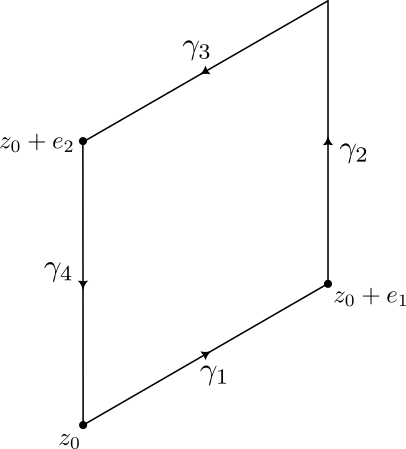
\includegraphics{Images/period_parallel_sum_of_poles.png}
        \caption{$\gamma_3(t) = \gamma_1(1 - t) + e_2$}
        \label{fig:period-parallel-sum}
    \end{figure}
    
    Therefore 
    \begin{align*}
        \frac{1}{2\pi i} \int_{\gamma_3} \frac{z f'(z)}{f(z) - a}dz &= -\frac{1}{2\pi i} \int_{\gamma_1} \frac{(z + e_2)f'(z + e_2)}{f(z + e_2) - a} dz\\ 
        &= -\frac{1}{2\pi i} \int_{\gamma_1}\frac{z f'(z)}{f(z) - a}dz - e_2 \cdot \frac{1}{2\pi i} \int_{\gamma_1} \frac{f'(z)}{f(z) - a} dz
    \end{align*}
    Therefore in particular
    $$ \frac{1}{2\pi i}\int_{\gamma_1} \frac{f'(z)}{f(z) - a} dz + \frac{1}{2\pi i} \int_{\gamma_3} \frac{f'(z)}{f(z) - a} = -e_2 \cdot \frac{1}{2\pi i}\int_{\gamma_1} \frac{f'(z)}{f(z) - a} dz$$
    Moreover the coefficient of $e_2$ is an integer since 
    \begin{align*}
        \frac{1}{2\pi i}\int_{\gamma_1} \frac{f'(z)}{f(z) - a} dz = \frac{1}{2\pi i}\int_{(f - a) \circ \gamma_1} \frac{1}{w} dw
    \end{align*}
    is simply the winding number of $(f - a) \circ \gamma_1$ with respect to 0.

    A similar thing happens with the left and right edges which we label $\gamma_2$ and $\gamma_4$ respectively. Therefore 
    \begin{align*}
        \frac{1}{2\pi i} \int_{\gamma} \frac{f'(z)}{f(z) - a} dz &= \sum_{i = 1}^4 \frac{1}{2\pi i} \int_{\gamma_i} \frac{f'(z)}{f(z) - a} dz\\
        &= e_1 \cdot \underbrace{-\frac{1}{2\pi i} \int_{\gamma_2} \frac{f'(z)}{f(z) - a} dz}_{\in \Z} + e_2 \cdot \underbrace{-\frac{1}{2\pi i} \int_{\gamma_1} \frac{f'(z)}{f(z) - a} dz}_{\in \Z}
    \end{align*}
    which is in $\Gamma$. 
\end{proof}

We immediately apply the results above to the case of $\wp(z)$.
\begin{theorem}\label{thm:wp-parametrises-ellptc-curve}
The right hand side of the equation satisfied by $(x, y) = (\wp(z), \wp'(z))$, namely 
\begin{equation}\label{eqn:p-func-diff-eqn}
    y^2 = 4x^3 - 20a_2x - 28a_4
\end{equation}
has 3 distinct roots. Moreover for all $(x, y)$ on this curve there exists a unique $z \in \C/\Gamma$ such that $(x, y) = (\wp(z), \wp'(z))$.
\end{theorem}
\begin{proof}
    Given $a \in \C$, we know that $\wp(z) = a$ has 2 roots in the period parallelogram and $\wp'(z) = a$ has 3 roots. This follows from \autoref{prop:num-zeros-poles-period-parallel} and the fact that $\wp(z)$ and $\wp'(z)$ have a double and triple pole (respectively) at $\omega \in \Gamma$. 

    We want to consider points $z \in \C$ such that $2z \in \Gamma$ but $z \notin \Gamma$. These points are interesting because they are exactly the points satisfying $z \equiv -z \bmod \Gamma$. It is easy to see that the only such points modulo $\Gamma$ are $e_1/2, e_2/2$ and $(e_1 + e_2)/2$. This is because if 
    $$2z = n_1 e_1 + n_2 e_2$$
    Then 
    $$z = \frac{n_1}{2}e_1 + \frac{n_2}{2}e_2$$
    so the only solutions modulo $\Gamma$ are when one or both of the coefficients of $e_1, e_2$ are $1/2$. If $z$ is any of the three points above then $z \equiv -z$ so
    $$\wp'(z) = \wp'(-z)$$
    On the other hand $\wp'$ is odd so for any $z$ at all we have
    $$\wp'(-z) = -\wp'(z)$$
    Therefore we conclude that $\wp'(z) = 0$ at the three points above. This means that at these three points the left hand side of the equation \eqref{eqn:p-func-diff-eqn} is 0 and thus $\wp(e_1/2), \wp(e_2/2), \wp((e_1 + e_2)/2)$ are zeroes of the right hand side. All that remains to show is that these are distinct. 

    Let $z_0$ be one of the 3 special points. Then we know that $\wp(z) - \wp(z_0)$ is 0 at $z_0$ and its derivative $\wp'(z)$ is also 0 at $z_0$. Therefore $\wp(z) - \wp(z_0)$ has a double root at $z_0$. Since $\wp(z) - a$ has exactly 2 roots for any $a$ we know that $\wp(z_0)$ cannot be achieved by any other point in the period parallelogram. Therefore the 3 zeroes to the equation are indeed distinct.

    For the second part of the statement, we already know the case for $y = 0$ (in particular since $(x, y)$ is on the curve, if $y = 0$ then $x$ would be a root of the right hand side and we have seen in this case $x$ is necessarily one of $\wp(e_1/2), \wp(e_2/2)$ and $\wp((e_1 + e_2)/2)$). Suppose $y \neq 0$. Then we know that $\wp(z) = x$ has 2 roots and since $\wp$ is even we know that $\wp(z) = \wp(-z)$ so the two roots are given by $z$ and $-z$. Since $y$ is not 0 we know that $2z \notin \Gamma$ so in particular $z$ and $-z$ are distinct. Looking at the equation, we can see that for a fixed $x$, there are exactly two choices of $y$ (provided $y \neq 0$) that only differ by a sign. Since $\wp'$ is odd, we know then that $y$ must be given by $\wp'(z)$ or $\wp'(-z)$. Thus for every $(x, y)$ on the curve, there exists a unique $z \in \C/\Gamma$ satisfying $(x, y) = (\wp(z), \wp'(z))$.
\end{proof}

